\documentclass[12pt]{article}
\usepackage[margin=1in]{geometry}
\usepackage{amsmath, amssymb}
\usepackage{fancyvrb}
\usepackage{color}
\usepackage{bussproofs}
\usepackage{graphicx}
\usepackage{fontspec}
\usepackage{setspace}
\doublespacing
\setmainfont{Times New Roman}

\fvset{%
  fontsize=\small,
  numbers=left
}

\makeatletter
\renewcommand{\Pr}[1]{\text{\textbf{Pr}}\left(#1\right)}
\renewcommand\subsection{\@startsection{subsection}{2}%
  \z@{-.5\linespacing\@plus-.7\linespacing}{.5\linespacing}%
  {\normalfont\scshape}}
\renewcommand\subsubsection{\@startsection{subsubsection}{3}%
  \z@{.5\linespacing\@plus.7\linespacing}{-.5em}%
  {\normalfont\scshape}}
\makeatother

\title{Urbanization in Shanghai}
\author{%
Arissa Li,
Evan Bergeron,
Lillian Cho,
Tiffany Lee
}
\date{\today}

\begin{document}
\maketitle
\section{NYC vs Shanghai: Urban Heat Island}

With global warming forecasts set to continue into the near and
no-so-near future, heat waves will become more and more likely to
occur over time. The Urban Heat Island metric (or UHI for short) is
typically defined as the temperature difference between urban,
suburban, and exurban areas. For instance, \cite{Tan2010} found that
over the last 30 years in Shanghai, the average mid-summer temperature
in urban districts has been increasing at an average rate of 0.073 K
per year, whereas surrounding exurban areas saw no substantial
change. That's a combined increase of urban mid-summer temperature by
more than 2 K.

Comparing results detailed in \cite{Gaffin2008} and \cite{Tan2010}, it
would appear that the UHI effect in NYC is still much more pronounced
than in Shanghai, though Shanghai is quickly catching up. This is a
pattern we see again and again. The majority of years between 1975 and
2010 saw a UHI intensity of roughly 2 to 2.5 K in NYC, with a handful
of years approaching 3 K. In Shanghai, we see an increase from a UHI
of 0.2 K in 1975 to a UHI of 1 K in 2000, with most of the 1990s
having a UHI of roughly 0.8 K.

According to \cite{Xia2014}, we have the following figures. We can see
that air quality and GDP growth are negatively correlated.

\begin{center}
\begin{tabular}{cccc}
  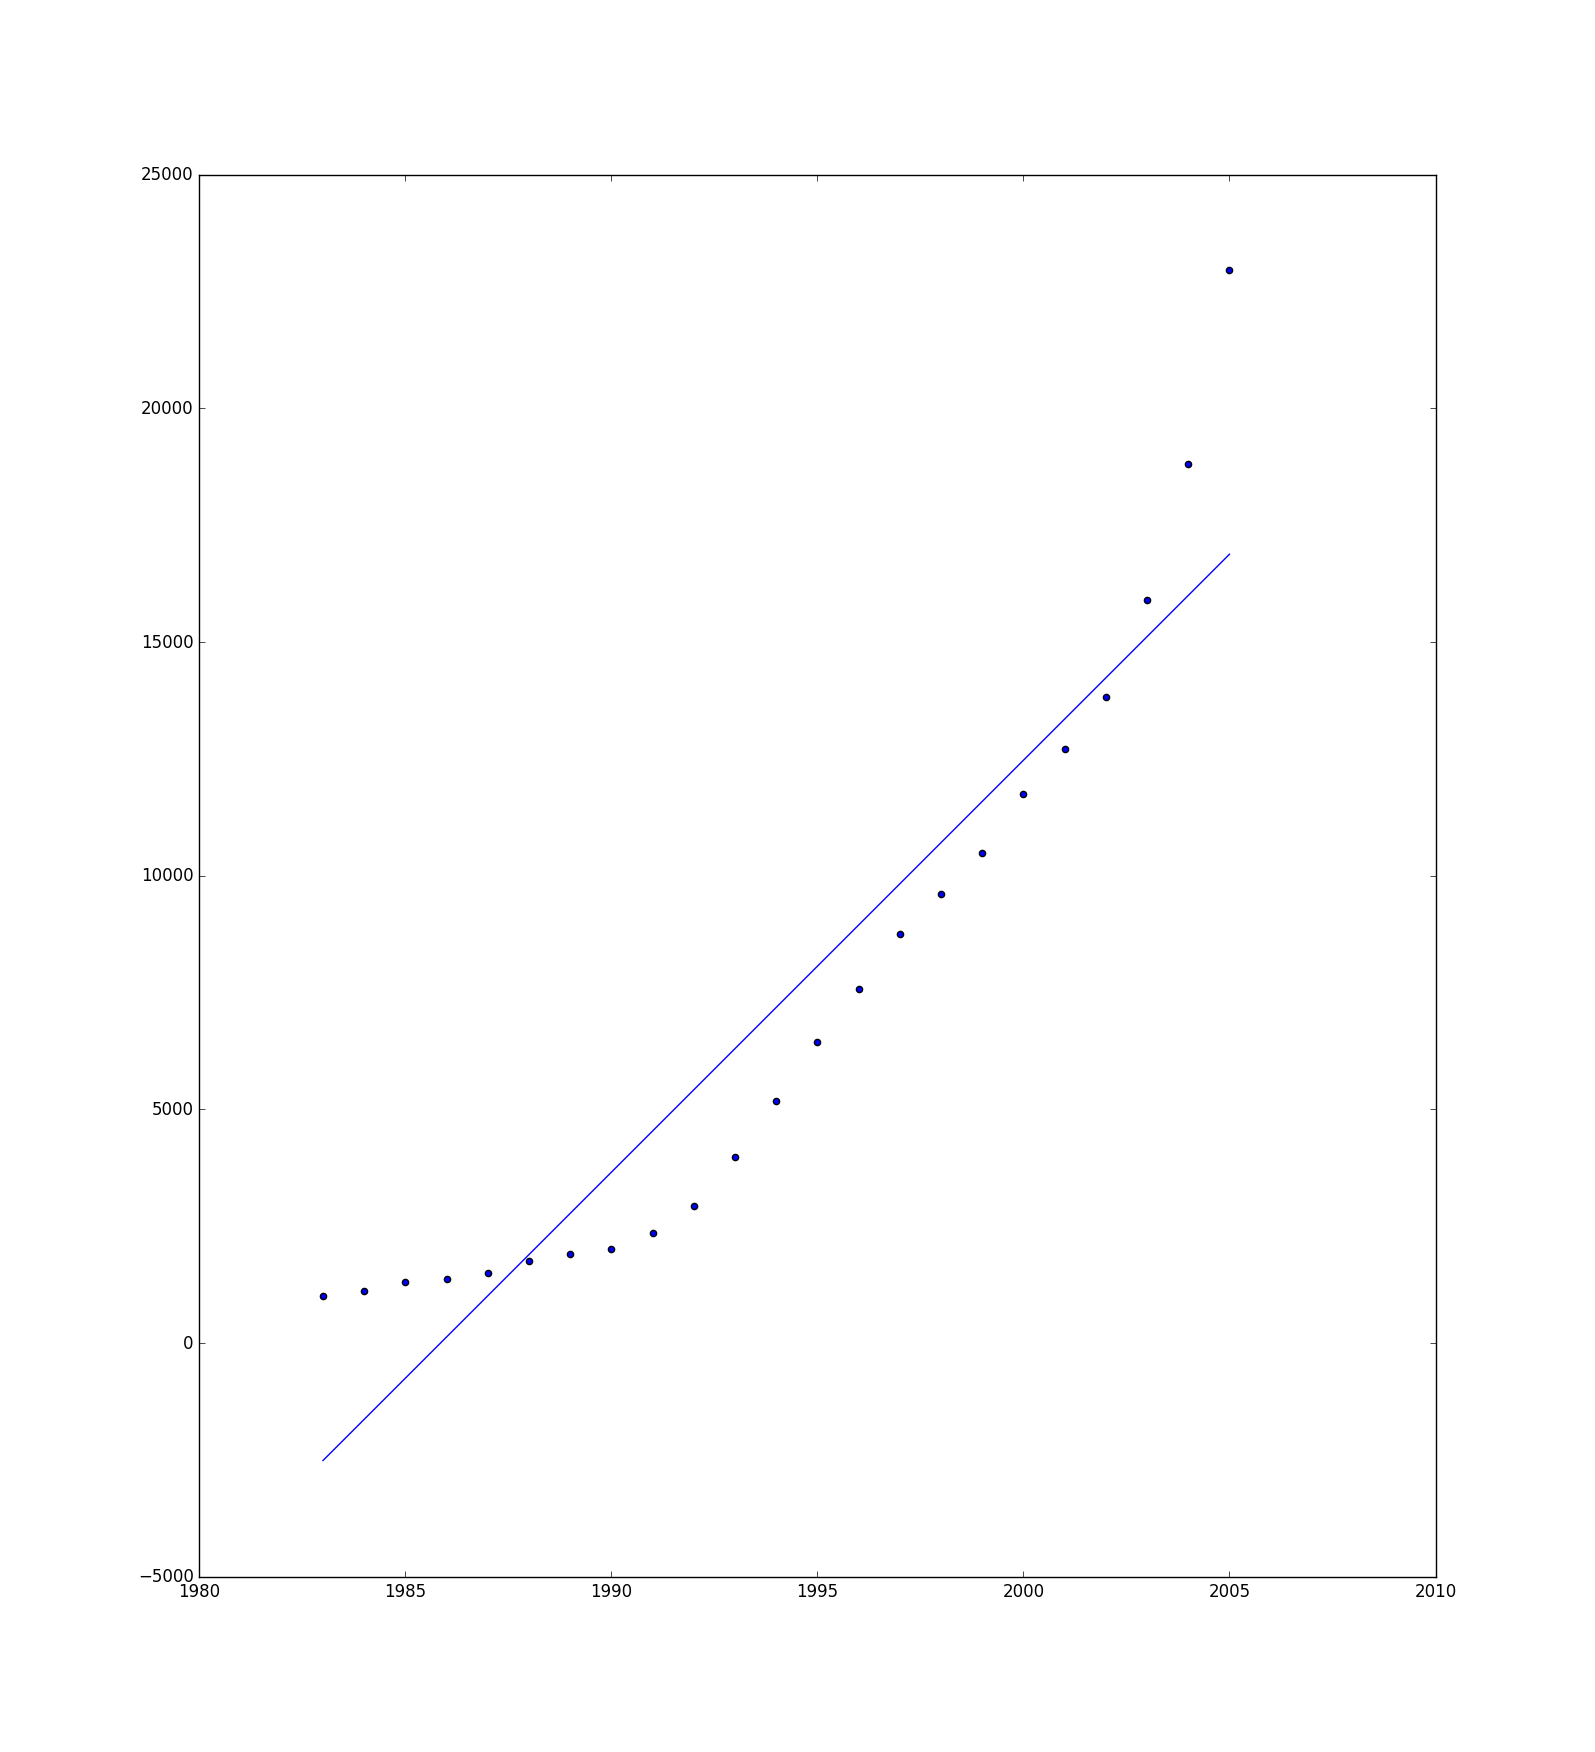
\includegraphics[width=0.2\textwidth]{img/growth_gdp}
& 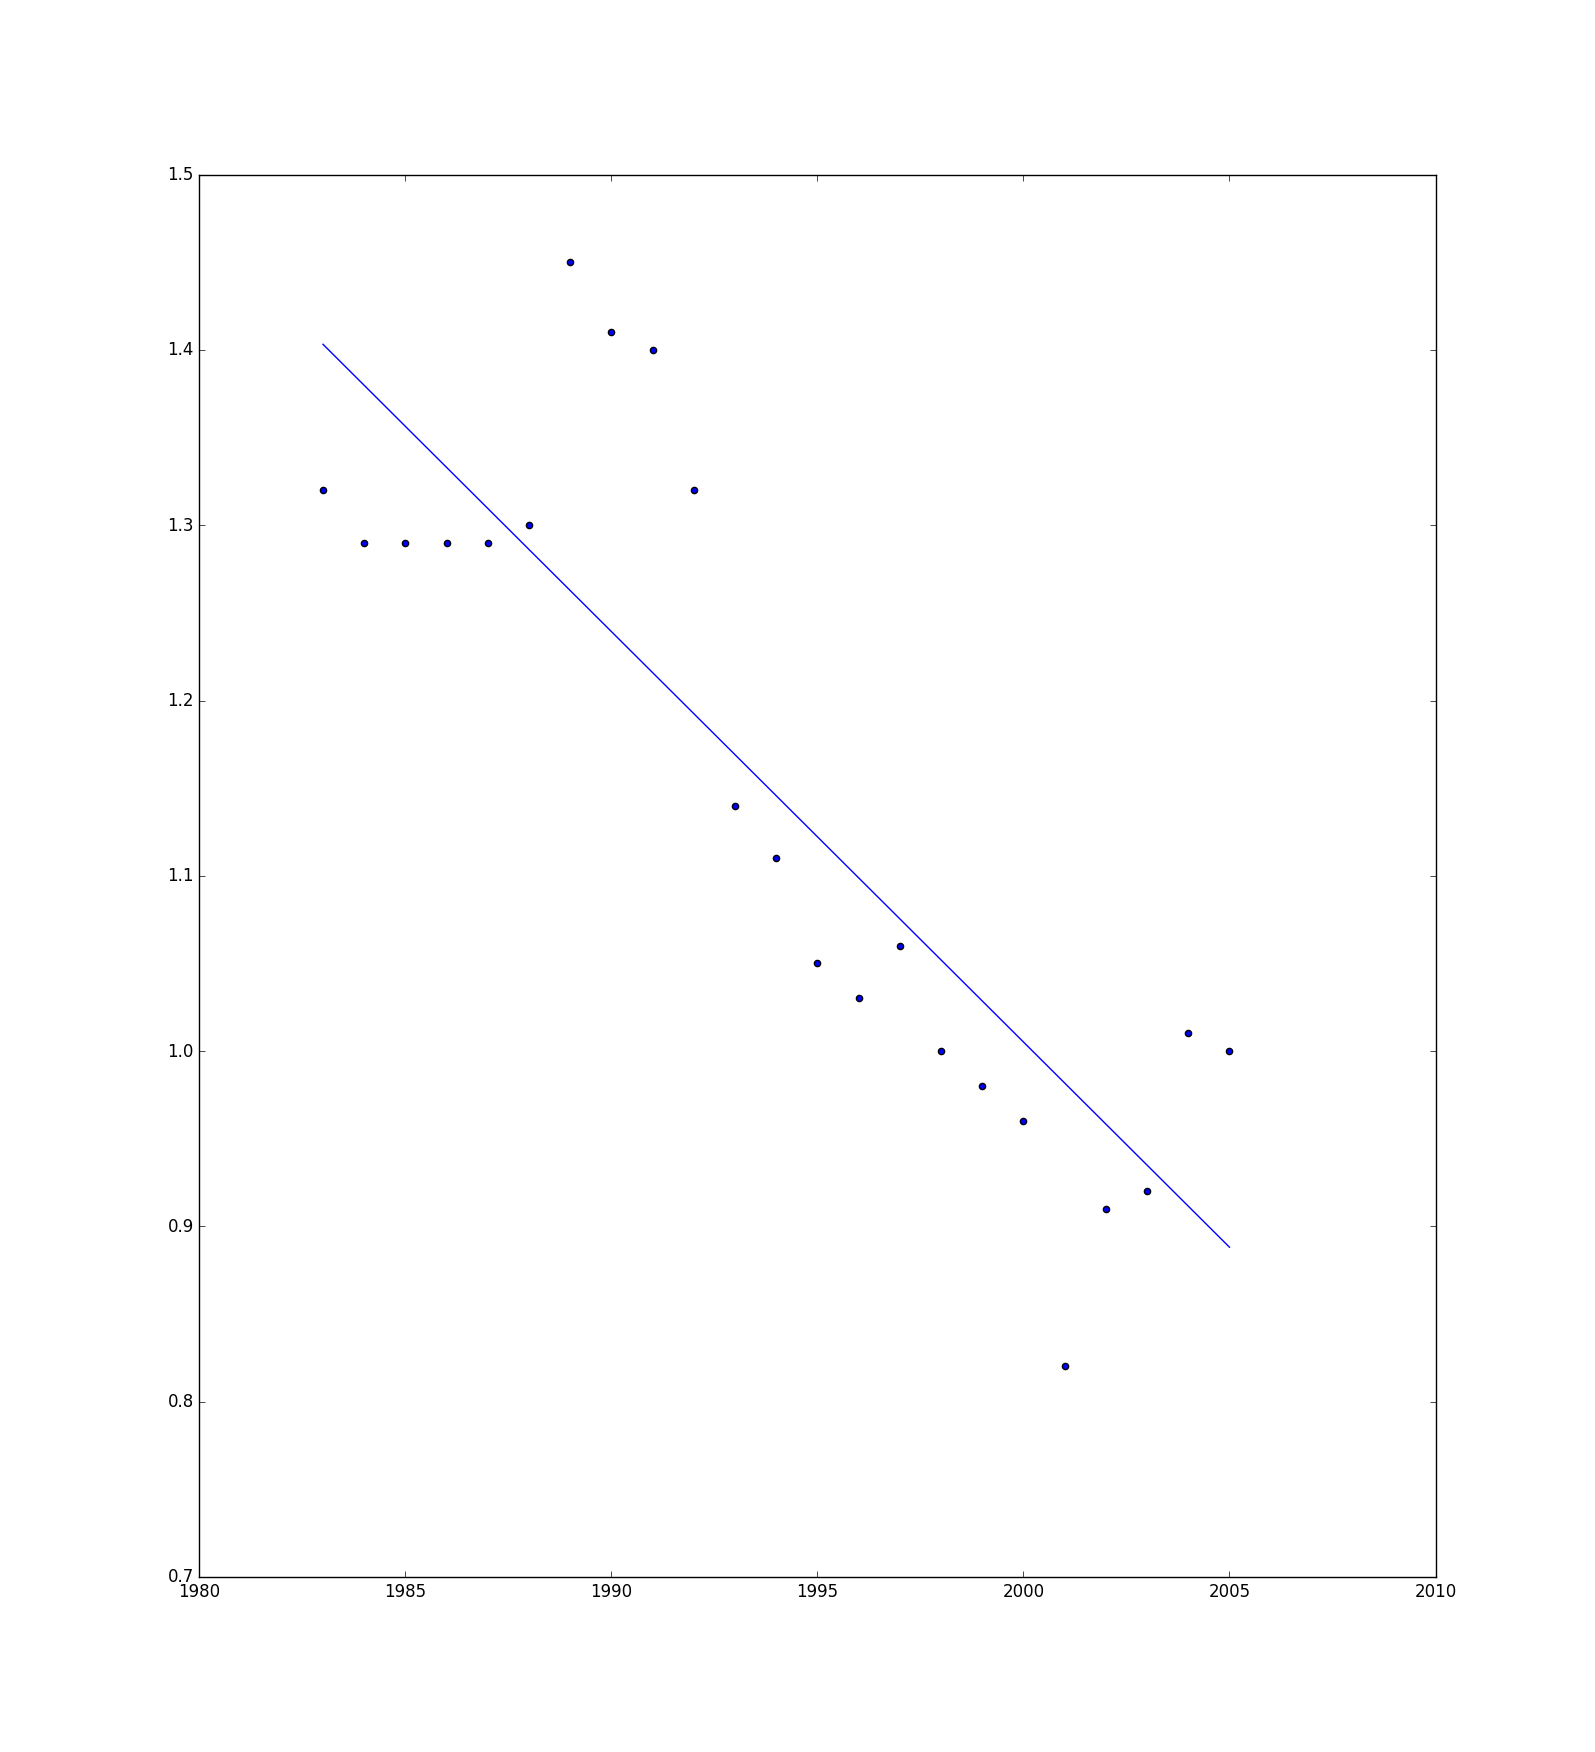
\includegraphics[width=0.2\textwidth]{img/air_quality}
& 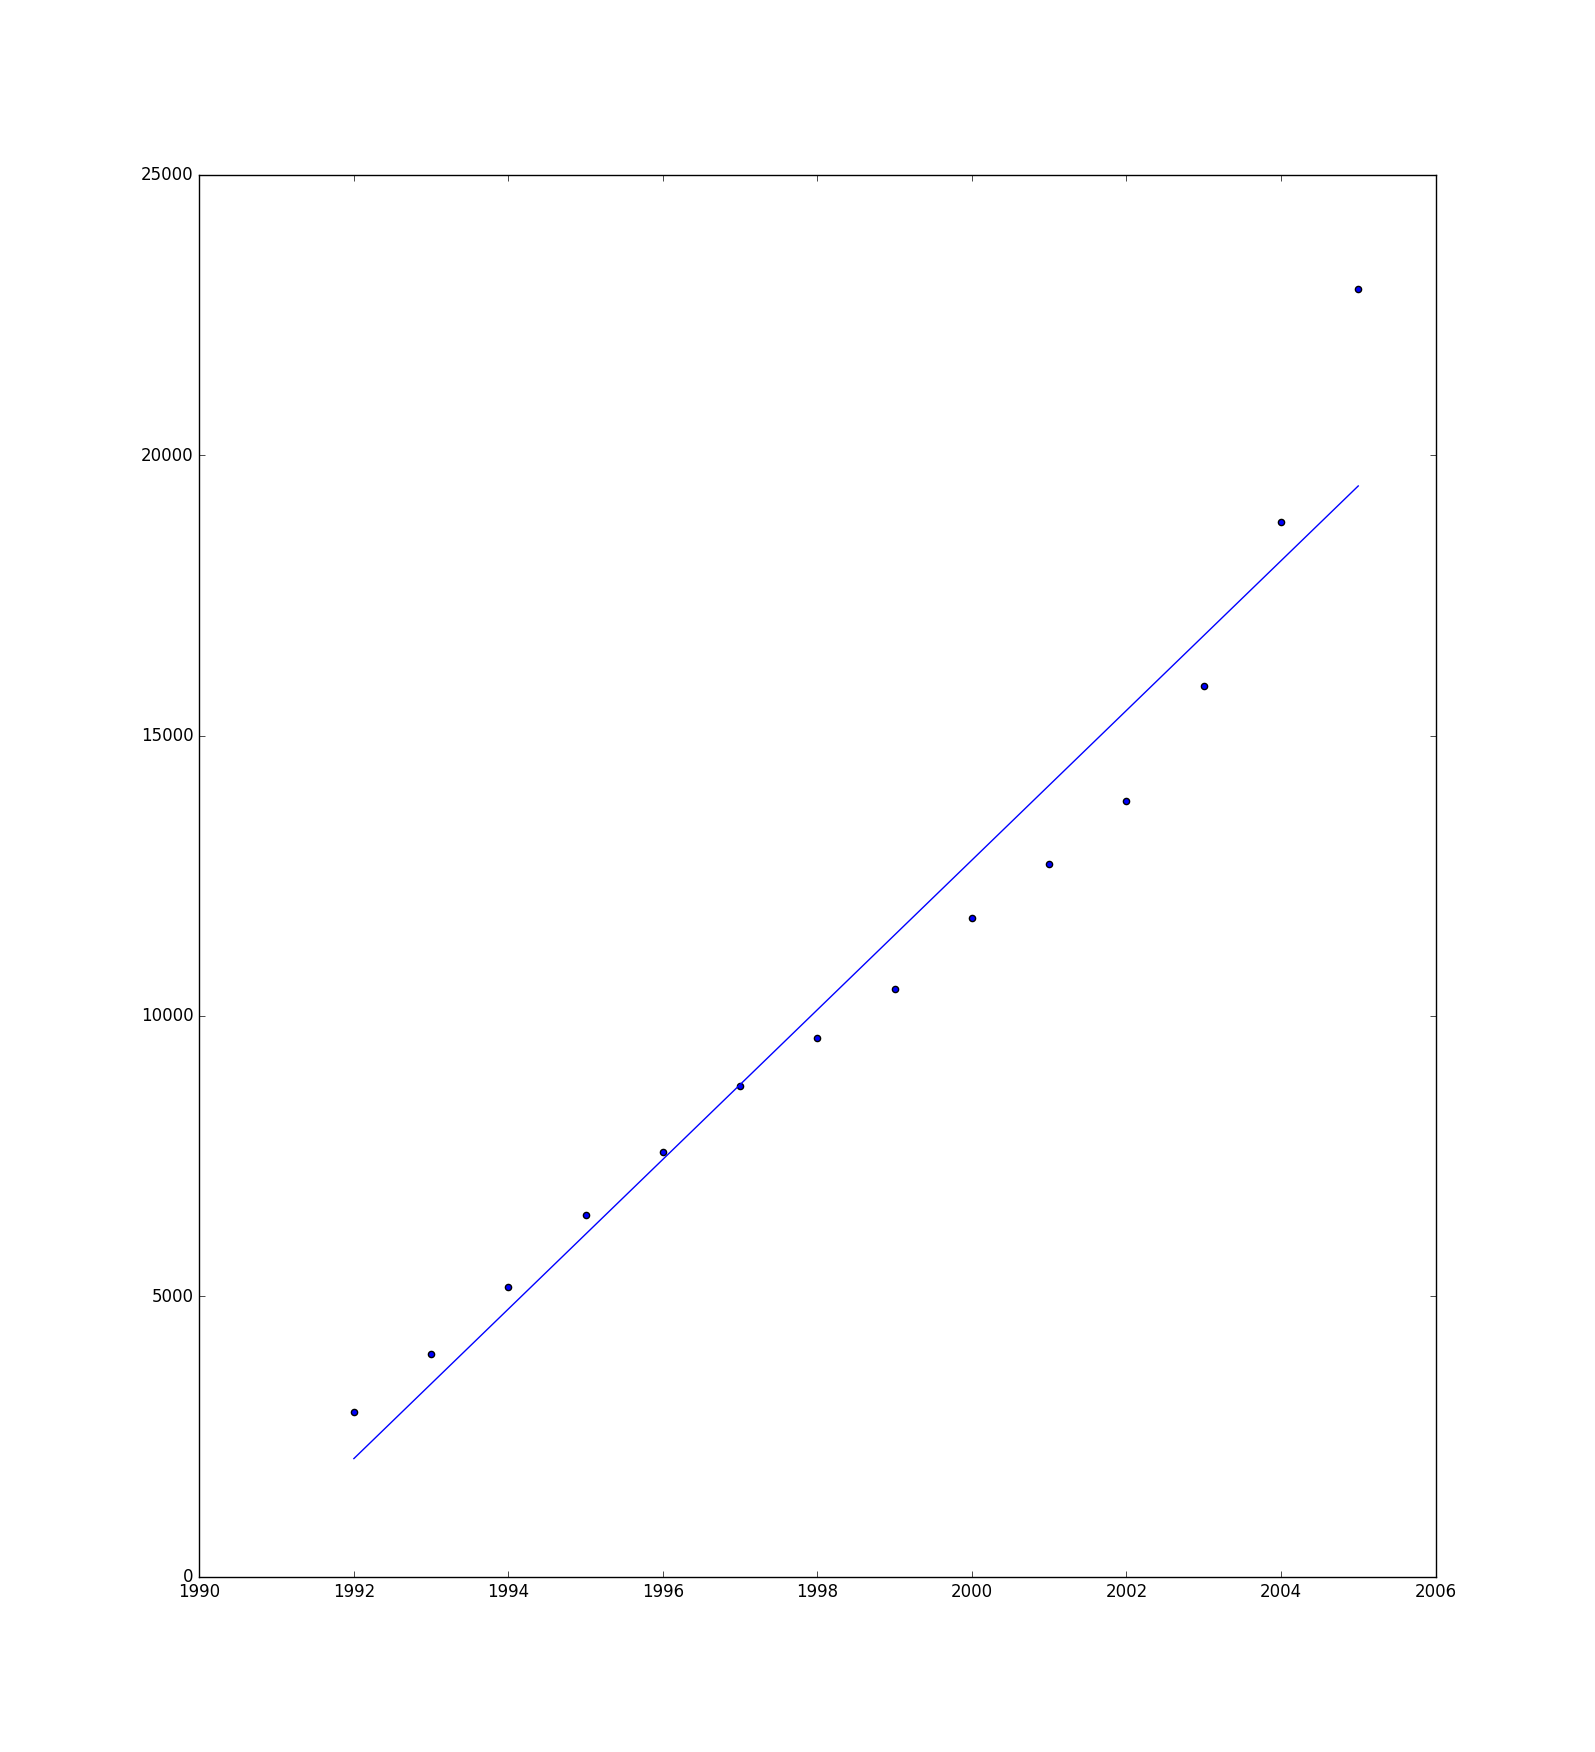
\includegraphics[width=0.2\textwidth]{img/growth_gdp_1991}
& 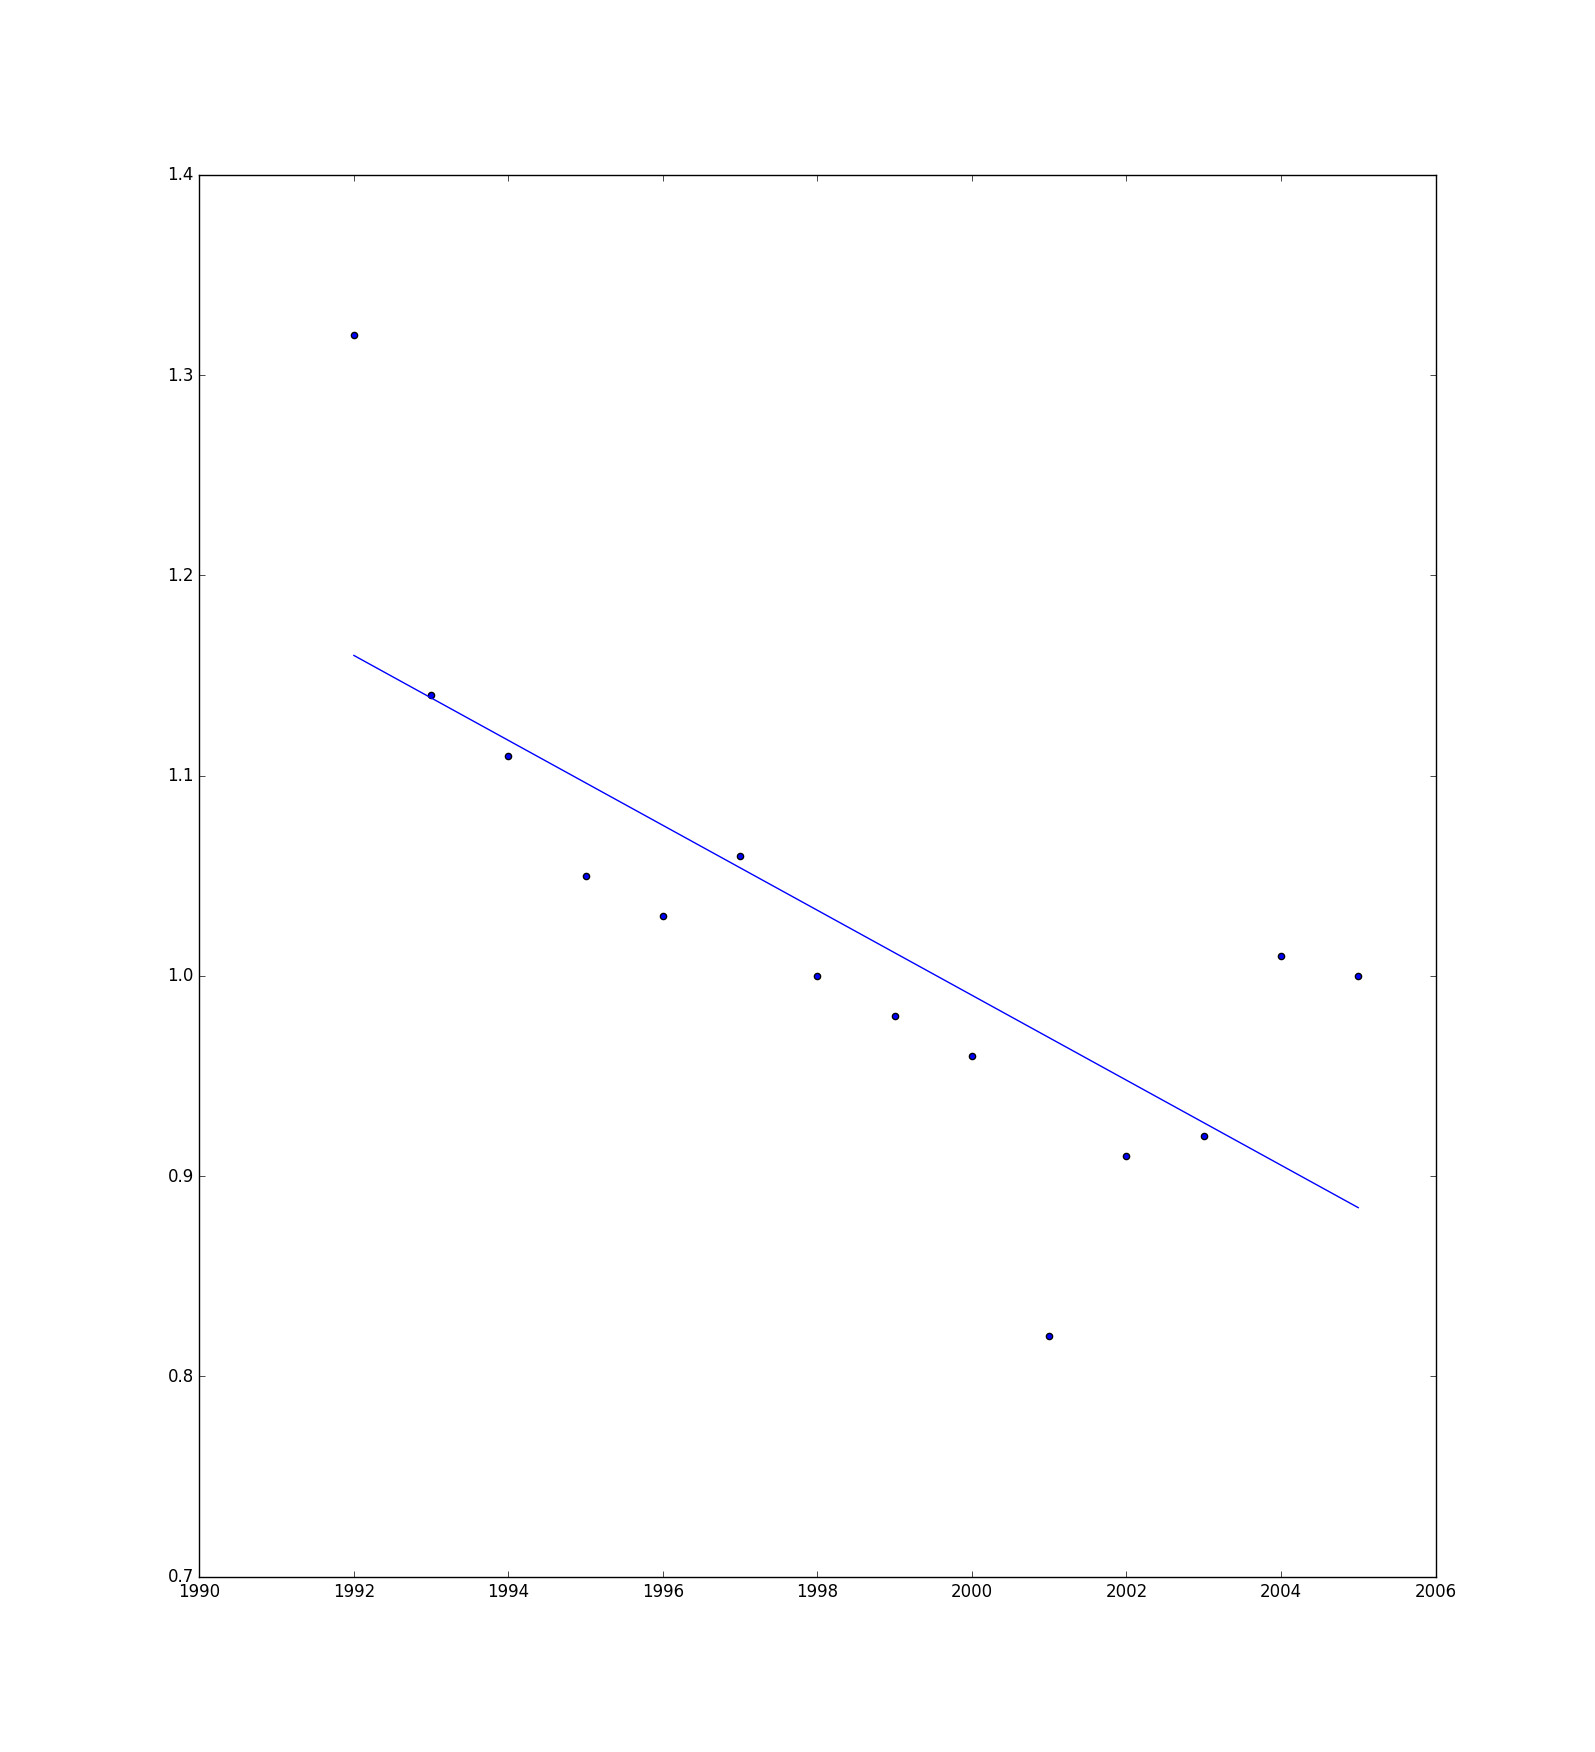
\includegraphics[width=0.2\textwidth]{img/air_quality_1991}\\
   GDP growth over time & Air quality over time 
&  GDP growth since 1991 & Air quality since 1991
\end{tabular}
\end{center}

\section{NYC vs Shanghai: Population}

Shanghai is a city whose population is substantially larger than any
American city. With a current population of well over 23 million
people, Shanghai has more inhabitants than many nations - including
Australia, Syria, and Greece.

The US population is still more urban, however. 62.7\% of US citizens
live within city limits,\cite{us-census:2011} whereas only 56\% of
Chinese citizen do. Additionally, the top 5 cities in the US represent
6\% of the total US population\cite{us-census:2011}. The top 5 Chinese
cities account for slightly less than 5\% of the Chinese population.

New York City is more population dense than Shanghai, with 10,194
people per square kilometer, versus 3,600 in Shanghai. This being
said, geographically, Shanghai occupies fully 7.5 times more land than
New York City.

From 2000 to 2010, Shanghai grew nearly as fast as any city in the
US. Shanghai grew by 37.53\% in population. In the US, the top three
cities grew by 41.83\%, 41.83\%, and 37.33\% (these were Las Vegas,NV,
Raleigh, NC, and Austin, TX)\cite{us-census:2011},
\cite{us-census:2001}. However, over this time period, Shanghai added
more than 6 million people; the cities of comparable growth rate in
the US grew by 575,504, 333,419, and 466,526, respectively.

Cars are much more common in the US, with 797 / 1000 people in the US
owning a car. In Chinese, only 205 / 1000 people own a car. Public
transit is much more common in China, with the Chinese government set
to spend more on high-speed trains in 2017 than the US Federal
Government will on all infrasture combined. Additionally, the US GDP
is still larger than that of China, only emphasizing the importance
public transit holds to the current Chinese government.

China has recently outpaced the US in economic inequality
\cite{Xie13052014}. The Gini coefficient is a statistical measure of
inequality. A polynomial fit approximation on data from 1965 to 2015
puts the turning point at slightly after the year 2000, at the end of
China's remarkably profitable 90s.

% bib stuff
\nocite{*}
% \addtocontents{toc}{\protect\vspace{\beforebibskip}}
\addcontentsline{toc}{section}{\refname}
\bibliographystyle{plain}
\bibliography{paper}

\end{document}
